% User verification
% - Biometria twarzy
% - Ogólna procedura weryfikacji 
% - Przetwarzanie wstępne 
% - Neuronowy extractor cech
%   * Klasyfikacja
%   * Triplet loss
%       - Negative examples sampling
% - Implementacja


\section[verification]{System weryfikacji użytkownika za pomocą biometrii twarzy}\label{sec:verification}

Kontrola dostępu, autoryzacja i identyfikacja osób jest wciąż otwartym problemem informatyki.
Implementacja polega zazwyczaj na podaniu przez osobę uwierzytelnianą kodu alfanumerycznego lub
zweryfikowaniu się kluczem(np. karta magnetyczna lub chipowa). Najbezpieczniejsze systemy
zabezpieczeń bazują jednak na cechach biometrycznych takie jak odcisk palca, tęczówka lub twarz.
Pomimo gorszej dokładności systemów bazujących na biometrii twarzy w porównaniu do innych, są one
bardzo często stosowane dzięki nieinwazyjności, bezkontaktowego dokonania pomiaru i popularności
w innych aplikacjach~\cite{FaceBiometric}.

\begin{figure}[h]
    \centering
    \includegraphics[width=1.\textwidth]{2-0_verification_general_drawio.pdf}
    \caption{\textbf{Proces weryfikacji użytkownika.} Proces rozpoczyna się od wykonania
    zdjęcia. Dalsze procesowanie składa się z etapu detekcji twarzy, wyznaczenia wektora cech twarzy(embeddingu) oraz porównania wektora z bazą danych.}
    \label{fig:proces_weryfikacji}
\end{figure}

Proces weryfikacji biometrią twarzy został pokazany na rysunku~\ref{fig:proces_weryfikacji}. Jak
w każdym innym tradycyjnym systemie kontroli dostępu potrzeba jest baza użytkowników. Tutaj dla
każdej z autoryzowanych osób przechowuje się wektor z wyznaczonymi cechami jej twarzy.
Wyznaczanie wektora zależy od zastosowanej metody i zostanie to omówione w
sekcji~\ref{sec:ekstraktor}. System na wejściu przyjmuje zdjęcie osoby poddawanej weryfikacji.
Technika wykonania zdjęcia zależy od realizacji systemu wizyjnego dlatego musi ono zostać
wstępnie przetworzone - usuwane jest zbędne tło i jest ono normalizowane(sekcja~\ref{sec:ekstrakcja_twarzy}). Następnie, powstały w
poprzednim kroku thumbnail twarzy przekształcany jest do tej samej przestrzeni wektorowej, do
której zostały zamienione twarze w bazie referencyjnej. W ten sposób w kolejnym kroku możemy w
prosty sposób porównać te wektory i stwierdzić czy weryfikacja jest pozytywna lub negatywna co
zostało omówione w sekcji~\ref{sec:verify_process}.


\subsection{Ekstrakcja twarzy i normalizacja obrazu}\label{sec:ekstrakcja_twarzy}
Wstępne przetwarzanie obrazu jest koniecznym krokiem w większości systemach wykorzystujących
wizje. Na zdjęciu na wejściu systemu oprócz twarzy osoby weryfikowanej mogą znajdować się 
w tle również twarze innych osób, dlatego w tym przypadku niezbędne będzie wykorzystanie metod
detekcji twarzy oraz algorytmów ciasnego dopasowania zdjęcia do jej konturów. Pod uwagę były
brane dwie architektury - MTCNN oraz RetinaFace. Wybór został ograniczony do tych dwóch głównie
ze względu na ich popularność, dobrą wydajność oraz to, że realizują to zadanie w sposób
end-to-end. Obie sieci z obrazu wejściowego wyekstrahują obszary, na których znajdują się twarze
i zwracają tę informację w postaci wektorów reprezentujących prostokąt na płaszczyźnie obrazu, w
którym znajduje się ciasno dopasowana twarz. Ze wszystkich twarzy wybierana jest ta, której
prostokąt ma największe pole - zakładamy, że użytkownik weryfikujący się znajduję się najbliżej
obiektywu kamery przez co jego twarz powinna być największa.

W tabeli~\ref{table:face_detector} pokazano porównanie dwóch detektorów twarzy. Z uwagi na to, że
ostatecznie największe znaczenie dla użytkownika końcowego ma dokładność całego systemu
porównujemy tutaj właśnie dokładność weryfikacji z wykorzystaniem ArcFace~\cite{Arcface} na
zbiorze danych LFW~\cite{DatasetLFW} w zależności od zastosowanego detektora twarzy. Wybrany
metoda będzie pracowała na urządzeniu o IoT dlatego porównujemy również szybkość modeli i 
rozmiar zapisanych wag na dysku. Czas inferencji jest średnim czasem jaki potrzebuje sieć na
przetworzenie jednego zdjęcia o rozdzielczości 320x240 pikseli. Uśredniona została detekcja na
wszystkich zdjęciach z zbioru LWF. Pomiary były wykonywane na urządzeniu RaspberryPi 4b
wykorzystując wszystkie dostępne rdzenie procesora.

\begin{table}[h]
\begin{center}
\begin{tabular}{cccc}
\hline
model & dokładność weryfikacji (\%)  &  czas inferencji (ms)  &   rozmiar na dysku (MB)  \\
\hline
MTCNN \cite{MTCNN}     & \num{99.83} & \num{83} & \num{1.9} \\ 
RetinaFace \cite{RetinaFace}   & \num{99.86}  & \num{112}& \num{1.8}  \\
\hline
\end{tabular}
\end{center}
\caption{\textbf{Porównanie detektorów twarzy}.}
\label{table:face_detector}
\vspace{-4mm}
\end{table}

W dalszej części pracy zostanie wykorzystany ekstraktor MTCC. Wybrano go głównie ze względu na jego
powszechność zastosowania w neuronowych metodach weryfikacji~\cite{Cosface,Arcface,Facenet}, szybkość oraz wystarczającą dokładność i wielkość na dysku. Na rysunku \ref{fig:ekstraktor_twarzy}
pokazano działanie wybranej architektury na przykładowych zdjęciach znajdujących sie w zbiorze
LFW. W celu analizy błędów jakie popełnia wybrany algorytm zostały pokazane
również przykłądy zdjęć z niewłaściwą detekcją - twarz została poprawnie wykryta ale nie jest ona
tą konkretną twarzą otagowaną w zbiorze danych. Obrazy te pokazują, że o ile zdjęcie zostanie wykonane w sposób właściwy, to jest, twarz osoby weryfikującej się będzie zajmowała największą część zdjęcia to błędy detektora nie powinny się propagować i wpływać na ostateczną wydajność weryfikacji.

\begin{figure}[H]
    \begin{center}
    \renewcommand\tabcolsep{1pt}
    {\bf Poprawna detekcja}
    \begin{tabular}{cc||cc||cc}
      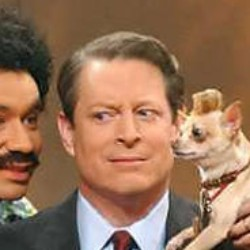
\includegraphics[width=.15\linewidth]{img/crop_examples/before/good/Al_Gore_0007.jpg} &
      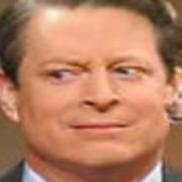
\includegraphics[width=.15\linewidth]{img/crop_examples/after/good/Al_Gore_0007.jpg} &
      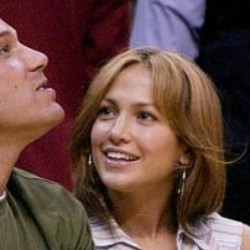
\includegraphics[width=.15\linewidth]{img/crop_examples/before/good/Jennifer_Lopez_0021.jpg} &
      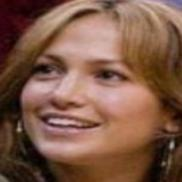
\includegraphics[width=.15\linewidth]{img/crop_examples/after/good/Jennifer_Lopez_0021.jpg} &
      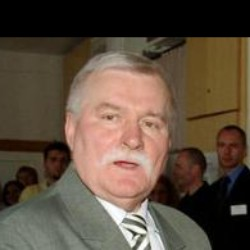
\includegraphics[width=.15\linewidth]{img/crop_examples/before/good/Lech_Walesa_0002.jpg} &
      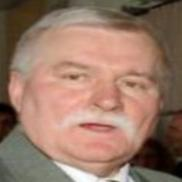
\includegraphics[width=.15\linewidth]{img/crop_examples/after/good/Lech_Walesa_0002.jpg} \\
    \end{tabular}
    {\bf Niepoprawna detekcja}
    \begin{tabular}{cc||cc||cc}
      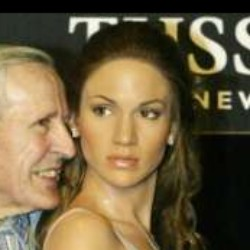
\includegraphics[width=.15\linewidth]{img/crop_examples/before/bad/Jennifer_Lopez_0020.jpg} &
      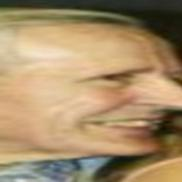
\includegraphics[width=.15\linewidth]{img/crop_examples/after/bad/Jennifer_Lopez_0020.jpg} &
      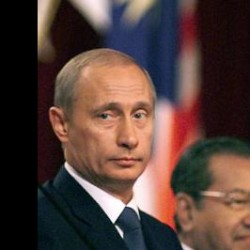
\includegraphics[width=.15\linewidth]{img/crop_examples/before/bad/Vladimir_Putin_0031.jpg} &
      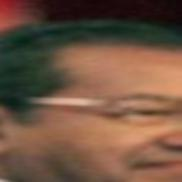
\includegraphics[width=.15\linewidth]{img/crop_examples/after/bad/Vladimir_Putin_0031.jpg} &
      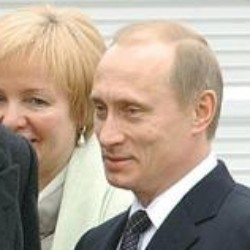
\includegraphics[width=.15\linewidth]{img/crop_examples/before/bad/Vladimir_Putin_0040.jpg} &
      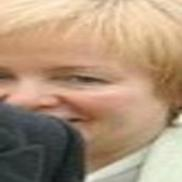
\includegraphics[width=.15\linewidth]{img/crop_examples/after/bad/Vladimir_Putin_0040.jpg} \\
    \end{tabular}
    \end{center}
    \caption{{\bf Przykłady działania ekstraktora twarzy.} Pokazane zostały tutaj wybrane przykłady prezentujące działanie ekstraktora twarzy.}
    \label{fig:ekstraktor_twarzy}
    \end{figure}

\subsection{Neuronowy ekstraktor cech} \label{sec:ekstraktor}

% W szczegółach zostaną omówione używana przez nas architektura w sekcji XXX
We współczesnych systemach weryfikacji zazwyczaj wykorzystuje się głębokie sieci konwolucyjne.
Pomijając na chwilę szczegóły modelu i traktując go jako czarną skrzynkę pokazano ogólną ideę
ekstraktora na rysunku~\ref{fig:ekstraktor_cech}. Głównym założeniem jest stworzenie systemu
end-to-end, którego wynikiem działania będzie wektor cech (embedding) \(f(x)\), wyznaczony z obrazu
wejściowego \(x\) przez rzutowanie go do pewnej przestrzeni cech \(\mathbb{R}^d\), w taki sposób,
że pewna funkcja odległości wyznaczona dla wszystkich zdjęć twarzy jest mała dla twarzy
należących do tych samych osób i duża dla różnych twarzy.
\begin{figure}[h]
    \centering
    \includegraphics[width=0.75\textwidth]{2-0_verification_ekstraktor_cech_drawio.pdf}
    \caption{\textbf{Struktura ekstraktora cech.} Ekstraktor składa się z wejścia, które w ogólnym przypadku może być paczką \(B\) przetworzonych wstępnie obrazów twarzy o wymiarach \( W \times H \times C\), głębokiej sieci konwolucyjnej i następującej po niej warstwie normalizacji. W rezultacie na wyjściu otrzymujemy \(B\) wektorów cech o wymiarach \(D\).}
    \label{fig:ekstraktor_cech}
\end{figure}


W literaturze można znaleźć dwie rodziny algorytmów trenujących głębokie sieci CNN ekstrahujące
cechy twarzy. Jedna wzorująca się na klasycznym podejściu stosowanym w treningu klasyfikatorów
obrazów. Najnowsze podejścia z tej rodziny algorytmów prezentujemy w sekcji
\ref{sec:klasyfikatory}. Druga gałąź algorytmów bazują treningu na optymalizacji wielu-klasowej
marginalnej funkcji straty (ang. multi-class classification hinge loss). Opisujemy je w
szczegółach w sekcji \ref{sec:tripletloss}

\subsubsection{Trening metodą optymalizacji klasyfikatora}\label{sec:klasyfikatory}

Wspólną cechą opisywanych tutaj metod jest trenowanie wielu-klasowego klasyfikatora, który
potrafi odróżnić różne osoby znajdujące się w zbiorze trenującym stosując funkcje Softmax. Głęboka sieć konwolucyjna mapuje wejściowe zdjęcie do takiej przestrzeni cech, że dodatkowy klasyfikator
trenowany na właśnie tych wektorach jest w stanie odróżnić i zidentyfikować osoby znajdujące się
na przykłądach trenujących. Podejście to ma dwie wady:

\begin{itemize}
  \item rozmiar macierzy liniowego przekształcenia klasyfikatora \(W \in \mathbb{R}^{d \times n}\) wzrasta liniowo wraz z liczbą osób \(n\). W niektórych zbiorach liczba ta sięga do nawet kilku milionów. 
  \item nauczone cechy są separowalne dla zamkniętego zadania klasyfikacji twarzy w zbiorze ale nie wystarczająco wyróżniające do zadania rozpoznawania z otwartą i nieograniczoną liczbą twarzy.
\end{itemize}

W literaturze znajduje się wiele odmian algorytmów bazujących na tym pomyśle. W centre
loss~\cite{Centreloss} wzbogacono funkcję straty o dwa komponenty. Pierwsza komponenta uwzględnia
wielkość odległości euklidesowej pomiędzy liczonej pomiędzy wektorami cech różnych klas, a druga
komponenta z kolei brała pod uwagę odległości wektorów należących do tych samych klas. Chciano w
ten sposób zapewnić inter-klasową kompaktowość reprezentacji oraz intra-klasową
rzadkość-reprezentacji. W CosFace~\cite{Cosface} dodano dodatkowo margines cosinusowy jako funkcje
kary, dodawanej do wektorów wychodzących bezpośredniego z sieci konwolucyjnej. W
ArcFace~\cite{Arcface} pomysł ten został jeszcze dalej rozwinięty jeszcze bardziej zwiększając moc
dyskryminującą wektorów cech. 

Ostanie usprawnienia, które zaszły w tej gałęzi algorytmów sprawiły, że wytrenowane w ten sposób CNN obecnie szczytują  w benchmarkach zarówno zadań weryfikacji, rozpoznawania jak i klasteryzacji osób. Bardzo dużą zaletą z perspektywy tej pracy jest duża popularność tych modeli - w sieci można znaleźć mnóstwo wysokiej implementacji oraz wysokiej jakości wytrenowanych modeli.  Niestety ze względu na to, że efektywny trening tą metodą wymaga obecności dużej liczby osób w zbiorze trenującym nie jest możliwe zastosowanie algorytmów z tej gałęzi do dotrenowywania modeli na urządzeniach użytkowników w ramach realizacji FL - nie jest możliwe, zebranie takiego zbioru na prywatnych urządzeniach nie naruszając prywatności danych.

\subsubsection{FaceNet}\label{sec:tripletloss}
Drugą gałęzią algorytmów trenujących ekstraktor cech są metody bezpośredniego uczenia się
embeddingu ze zdjęcia. W szczególności interesującą architekturą jest FaceNet~\cite{Facenet}.
Metoda ta bazuje na nauczeniu sieci generowania z obrazu embeddingu od razu znajdującego się w przestrzeni Euklidesowej. Traktując model jako czarną skrzynkę (rysunek~\ref{fig:facenet_idea}), sieć jest trenowana tak, żeby kwadrat odległości \(L_2\) między dwoma embeddingami
odpowiadał bezpośrednio podobieństwu twarzy: twarze tej samej osoby mają małe wzajemne
odległości, a twarze różnych osób duże. Kiedy embedding został wyznaczony, realizacja
zadania weryfikacji jest prosta - wystarczy zastosować progowanie na dystansie pomiędzy dwoma
wektorami cech. Generowane embeddingi w szczególności powinny być skuteczne w zadaniu weryfikacji, wykorzystywana funkcja straty zaczęca aby wszystkie twarze jednej osoby zostały projektowane do wspólnego punktu w przestrzeni embeddingów jednocześnie wymuszając  margines pomiędzy jedną, a pozostałymi osobami.

\begin{figure}[h]
    \centering
    \includegraphics[width=0.75\textwidth]{facenet_idea_drawio.pdf}
    \caption{\textbf{Struktura modelu.} Model Facenet składa się z warstwy wejściowej, głębokiej sieci konwolucyjnej (DCNN) oraz następującej po niej normalizacji \(L_2\), która w rezultacie zwraca embedding. Na końcu podczas trenowania dołączana jest warstwa z funkcją straty - triplet loss.}
    \label{fig:facenet_idea}
\end{figure}

\paragraph{Triplet loss}
Embedding jest reprezentowany przez \(f(x)\in\mathbb{R}^d\). Enkoduje on zdjęcie \(x\) w
\(d\)-wymiarową przestrzeń Euklidesową. Dodatkowo, zostaje wprowadzone ograniczenie aby embedding
znajdował się w \(d\)-wymiarowej hipersferze, tj. \(\|f(x)\|_2=1\). Funkcja straty ma zmusić aby
obraz \emph{anchor}) $x_i^a$ będącym zdjęciem pewnej osoby znajduje się bliżej do wszystkich
innych zdjęć \(x_i^p\) (\emph{pozytywne}) tej samej osoby niż wszystkich inny zdjęć \(x_i^n\) (\emph{negatywne}) innych osób. Zostało to zwizualizowane na rysunku~\ref{fig:triplet_loss}. Musi więc zachodzić następujący warunek:

\begin{align}\label{eq:triplet_constraint}
  \|f(x_i^a) - f(x_i^p)\|_2^2 + \alpha &< \|f(x_i^a) - f(x_i^n)\|_2^2\;
\end{align}
gdzie $\alpha$ jest wymuszonym marginesem odległości pomiędzy przykładami pozytywnymi i negatywnymi.

Funkcja straty, która wymusza spełnienie tego warunku jest definiowana jest przez $L=$
\begin{equation}\label{eq:triplet_loss}
  \sum_i^N\left[\left\|f(x_i^a)-f(x_i^p)\right\|_2^2 -
                  \left\|f(x_i^a)-f(x_i^n)\right\|_2^2+\alpha\right]_+\;.
\end{equation}


\begin{figure}[h]
    \centering
    \includegraphics[width=0.75\textwidth]{triplet_loss_drawio.pdf}
    \caption{Funkcja straty \textbf{triplet loss.} minimalizuje odległości pomiędzy przykładem \emph{anchor}, a przykładem \emph{pozytywnym}, z których oba są tą samą osobą i maksymalizuje odległość pomiedzy przykładami o różnych personaliów - \emph{anchor} i \emph{negatywny}}
    \label{fig:triplet_loss}
\end{figure}


\paragraph{Selekcja trójek}
 Krytycznie ważny jest sposób przykładów wchodzących do trójek. Przede wszystkim przykłady
 powinny być trudne dla sieci tak aby warunek~\ref{eq:triplet_constraint} był naruszany i sieć
 mogła otrzymać sygnał trenujący. Z drugiej strony selekcja najtrudniejszych przykładów będzie
 prowadziła do wchodzenia w lokalne minima na początku treningu i w konsekwencji wolną zbieżność.
 Autorzy proponują żeby dla każdej pary \(x_i^a\),\(x_i^p\) wybrać takie \(n_i^n\) aby
 \begin{equation}\label{eq:semi_hard}
  \left\|f(x_i^a)-f(x_i^p)\right\|_2^2<\left\|f(x_i^a)-f(x_i^n)\right\|_2^2\;.
 \end{equation}
 Takie przykłady negatywne są \emph{pół-trudne}, znajdują się dalej od przykładu anchor niż przykład pozytywny ale wciąż są w pewny sposób wymagające ponieważ wciąż znajdują się blisko pary \(x_i^a\),\(x_i^p\) - wciąż znajdują się w marginesie \(alpha\).

Podejście to jest wielce obiecujące jednak nie jest wolne od wad:
\begin{itemize}
  \item przy większych zbiorach danych występuje eksplozja kombinacji liczby trójek twarzy co prowadzi do znacznego wzrostu w liczbie kroków optymalizacji,
  \item znajdowanie \emph{pół-trudnych} przykładów do trójek jest zadaniem conajmniej kłopotliwym,
  \item w mini-batchu powinna być odpowiednio duża ilość par anchor-pozytywny co narzuca dodatkowe wymagania co do użytego zbioru trenującego,
  \item metada w praktyce wymaga ekstremalnie długich czasów treningu,
  \item z punktu tej pracy istotną wadą jest brak dobrych implementacji i dostępnych wytrenowanych modeli. 
\end{itemize}

FaceNet jest bardzo obiecującym podejściem do trenowania ekstraktora cech twarzy. Z punku widzenia tej pracy ogromną zaletą jest brak potrzeby treningu klasyfikatora. Model do wykonania kroków optymalizacji nie potrzebuje znać wszystkich  osób znajdujących się w zbiorze trenującym co daję nadzieje na możliwe zastosowanie tej metody w późniejszym douczaniu modelu na urządzeniach użytkownika. Użytkownik przez interakcje z urządzeniem tworzy przykłady pozytywne oraz anchor - jedynym problemem wydaje się być tworzenie przykładów negatywnych jednak problem ten zostanie poruszany w dalszych rozdziałach.


\subsubsection{Podsumowanie ekstraktorów cech twarzy}\label{sec:extraktor-podsumowanie}
 Wybór odpowiedniego modelu ekstrakcji cech jest kluczowe w implementacji systemu systemu. Z jednej strony bardzo ważne jest aby wybrać możliwie jak najskuteczniejszą metodę, z drugiej trzeba wziąć pod uwagę ograniczenia jakie narzuca na nas Federated Learning. W tabeli~\ref{table:losscompare} znajduje się porównanie metod ze względu na ich wydajność w zadaniach weryfikacji.

 \begin{table}[ht!]
  \begin{center}
  \begin{tabular}{cccc}
  \hline
  Loss Functions   & LFW & CFP-FP & AgeDB-30 \\
  \hline
  Softmax              & 99.08 & 94.39 & 92.33 \\
  CosFace & 99.33 & - & - \\
  SphereFace  & 99.42 & - & - \\
  ArcFace      & {\bf 99.53} & {\bf 95.56} & {\bf 95.15}\\
  \hline
  Triplet (FaceNet)       & 98.98 & 91.90 & 89.98 \\
  ArcFace+Triplet (FaceNet)      & 99.50 & 95.51 & 94.40  \\
  \hline
  \end{tabular}
  \end{center}
  \vspace{-2mm}
  \caption{\textbf{Wyniki weryfikacji} ($\%$) w zależności od użytej funkcji straty na trzech benchmarkach LFW, CFP-FP oraz AgeDB-30. Jako DCNN był wykorzystany ResNet50. Umieszczone wyniki są wynikami raportowanymi przez autorów poszczególnych metod.}
  \label{table:losscompare}
  \vspace{-3mm}
  \end{table}

  Najlepsze metody zdają się bazować na treningu klasyfikatora. Jednak ze względu specyficzności
  FL nie mogą być one stosowane w dotrenowywaniu modeli na urządzaniach IoT. Z drugiej strony wynik otrzymany przez FaceNet jest wciąż bardzo dobry. Pod względem szybkości wszystkie brane pod uwagę metody są sobie równe - finałowa szybkość zależy od użytej pod spodem architektury DCNN, której wybór może być niezależny od wyboru funkcji straty. 

  Ostatecznie FaceNet jest jedyną metodą nadająca się do zastosowania w naszym specyficznym środowisku produkcyjnym dlatego zostanie ona wykorzystana w dalszych etapach tej pracy.
  

% \begin{align}\label{eq:triplet_dystant}
    % \left\Vert f(x_i) - f(x_j) \right\Vert_q^p < \alpha
% \end{align}

\subsection{Procedura weryfikacji przy wykorzystaniu sieci neuronowych}\label{sec:verify_process}

Mając model obliczający wektory cech z obrazów można przejść do kolejnego i ostatniego kroku
procesu weryfikacji - decyzji co do wyniku. Weryfikacja twarzy jest zadaniem przyrównania twarzy
kandydata do innej i sprawdzenie czy nastąpiło ich dopasowanie. Jest to mapowanie
jeden-do-jednego: należy sprawdzić czy jest to ta sama osoba.

Mając na wejściu systemu dwa zdjęcia \(x_i\) oraz \(x_j\) wynik weryfikacji będzie wyznaczany następująco:

\begin{align}\label{eq:ekstraktor_weryfikacja}
\text{weryfikacja jest}\begin{cases}
    \text{pozytywna},& \text{jeśli } d(f(x_i), f(x_j) < \alpha \\
    \text{negatywna},              & \text{w.p.p}
\end{cases}
\end{align}

gdzie \(f(x)\) jest wektorem cech obrazu \(x\), opisanym w sekcji
\ref{sec:ekstraktor}, \(\alpha\) jest marginesem, \(d(f_1, f_2)\) jest pewną funkcją dystansu liczoną pomiędzy wektorami wyznaczanymi przez \(f(x)\). W przypadku FaceNet funkcja \(d\) jest po prostu odległością \(L_2\).

Parametr \(\alpha\) jest wybierany na podstawie cross-walidacji modelu na zbiorze walidacyjnym. 
